% !TeX spellcheck = cs_CZ
%{\tikzset{external/prefix={tikz/FYZII/}}
% \tikzset{external/figure name/.add={ch21_}{}}
%---------------------------------------------------------------------------------------------------
% file fey2ch21.tex
%---------------------------------------------------------------------------------------------------
%=========================== Kapitola: Řešení Maxwellových rovnic s proudy a náboji ================
\setchaptertoc
\chapter{Řešení Maxwellových rovnic s proudy a náboji}\label{fyz:IIchapXXI}

  \section{Světlo a elektromagnetické vlny}\label{fyz:IIchapXXIsecI}
  \section{Kulové vlny z bodového náboje}\label{fyz:IIchapXXIsecII}
  \section{Obecné řešení Maxwellových rovnic}\label{fyz:IIchapXXIsecIII}
  \section{Pole oscilujícího dipólu}\label{fyz:IIchapXXIsecIV}
  \section{Potenciály pohybujícího se náboje. Liénardovo a Weichertovo obecné 
  řešení}\label{fyz:IIchapXXIsecV}
  \section{Potenciály náboje pohybujícího se rovnoměrně. Lorentzův vzorec	
  }\label{fyz:IIchapXXIsecVI}
  \section{Příklady a cvičení}\label{fyz:IIchapXXIsecVII}



    \begin{figure}[ht!] %\ref{fyz:fig576}
      \centering
      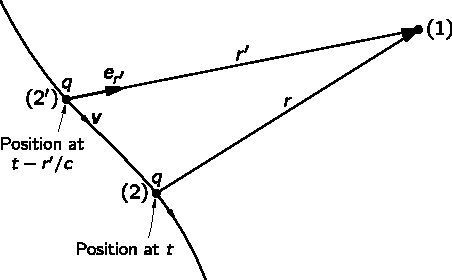
\includegraphics[width=0.7\linewidth]{fyz_fig576.pdf}
      \caption{
               (\cite[s.~707]{Feynman02})}
      \label{fyz:fig576}
    \end{figure}

    \begin{figure}[ht!] %\ref{fyz:fig577}
      \centering
      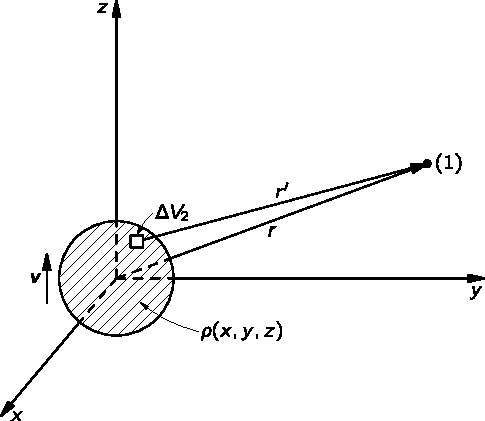
\includegraphics[width=0.7\linewidth]{fyz_fig577.pdf}
      \caption{
               (\cite[s.~707]{Feynman02})}
      \label{fyz:fig577}
    \end{figure}
    
    \begin{figure}[ht!] %\ref{fyz:fig578}
      \centering
      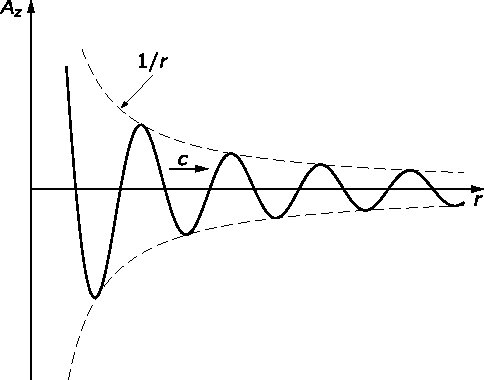
\includegraphics[width=0.7\linewidth]{fyz_fig578.pdf}
      \caption{
               (\cite[s.~707]{Feynman02})}
      \label{fyz:fig578}
    \end{figure}

    \begin{figure}[ht!] %\ref{fyz:fig579}
      \centering
      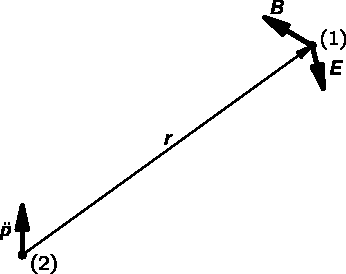
\includegraphics[width=0.7\linewidth]{fyz_fig579.pdf}
      \caption{
               (\cite[s.~707]{Feynman02})}
      \label{fyz:fig579}
    \end{figure}

    \begin{figure}[ht!] %\ref{fyz:fig580}
      \centering
      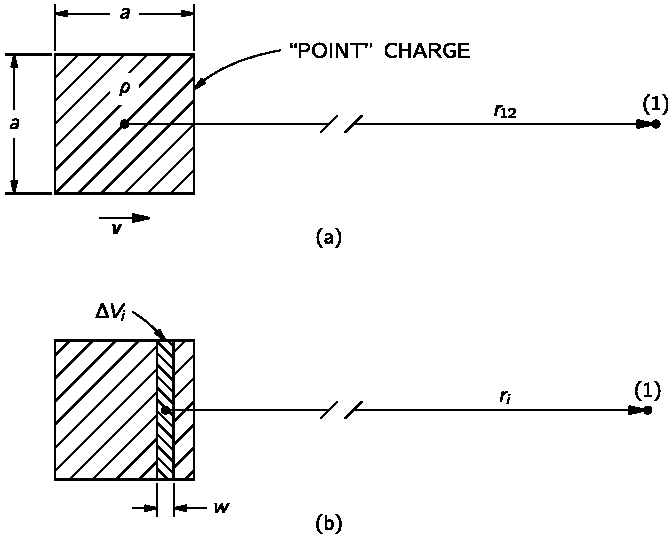
\includegraphics[width=0.7\linewidth]{fyz_fig580.pdf}
      \caption{
               (\cite[s.~707]{Feynman02})}
      \label{fyz:fig580}
    \end{figure}
    
    \begin{figure}[ht!] %\ref{fyz:fig581}
      \centering
      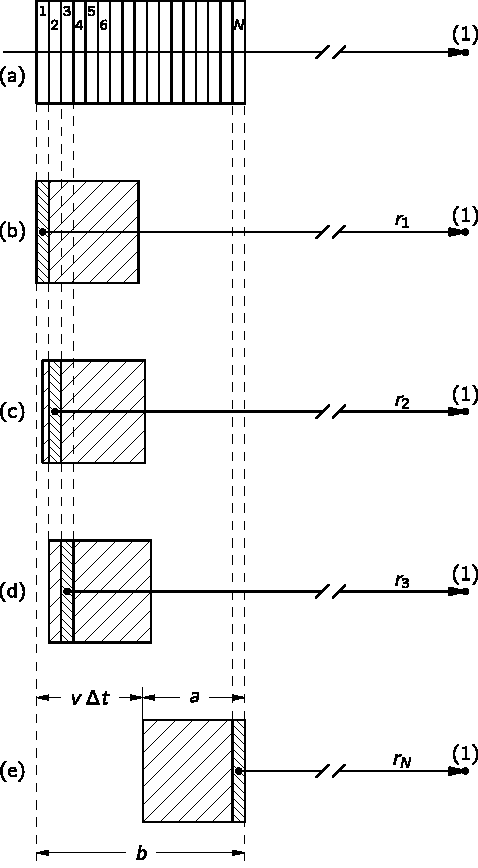
\includegraphics[width=0.7\linewidth]{fyz_fig581.pdf}
      \caption{
               (\cite[s.~707]{Feynman02})}
      \label{fyz:fig581}
    \end{figure}

    \begin{figure}[ht!] %\ref{fyz:fig582}
      \centering
      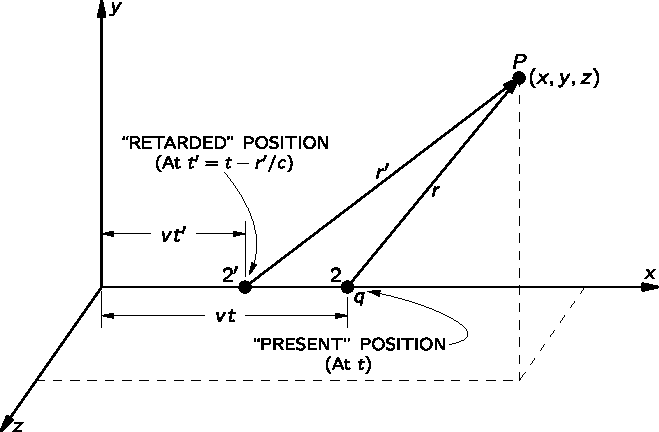
\includegraphics[width=0.7\linewidth]{fyz_fig582.pdf}
      \caption{
               (\cite[s.~707]{Feynman02})}
      \label{fyz:fig582}
    \end{figure}

    \todo[inline]{Kapitola fey2ch21 je nedodělaná, obsahuje pouze obrázky}
%} %tikzset
%---------------------------------------------------------------------------------------------------
